
\begin{frame}
\frametitle{A Little Background}
%\lipsum[1]

\begin{itemize}
\item Created by: Guido van Rossum, 1989-1991
\item Why: The creator wanted something easy to use.
\item Is it really that easy? Yes (and no)
\item Very readable with little memory management.
\item \url{https://people.sc.fsu.edu/~jburkardt/}
\item \url{https://docs.python.org/3/tutorial/index.html}
\item \url{https://www.tutorialsteacher.com/python}
\item \url{https://www.w3schools.com/python/default.asp}
\item \url{https://www.tutorialspoint.com/python/} $\longleftarrow$ great place to start.
\end{itemize}

\end{frame}

\begin{frame}
\frametitle{A Little More About Python}

\begin{itemize}
\item Python2 $\longrightarrow$ Python3; support for Python2 will end 2020.
\item This workshop is exclusively on Python3 $\longrightarrow$ refer to just Python
\item Python is fully object oriented. Everything is considered object.
\item Famous for AI and machine learning $\longrightarrow$ Pytorch, Keras, TensorFlow
\item Interpreter language but can be compiled $\longrightarrow$ Cython, Numba
\item Very well documented. Every module/libraries are documented online.
\item Package management by package installer $\longrightarrow$ pip, pip3
\item pip $\longrightarrow$ \url{https://pypi.org/project/pip/}
\item \textbf{Py}thon \textbf{P}ackage \textbf{I}ndex $\longrightarrow$ pypi, \url{https://pypi.org/}
\item \url{https://github.com/} $\longleftarrow$ another place to look.
\end{itemize}

\end{frame}

\begin{frame}
\frametitle{About Anaconda}
\begin{itemize}
\item No, its not a different programming language.
\item Anaconda is a \emph{complete environment} for Python programming.
\item Most major scientific package (NumPy, SciPy etc) are included.
\item Package installer \emph{conda}
\lstinputlisting[language=bash, firstline=5, lastline=5, numbers=none]{./install-commands.txt}
\item \url{https://www.anaconda.com/}
\end{itemize}

\end{frame}
\begin{frame}[fragile]
\frametitle{About programming}
\begin{figure}
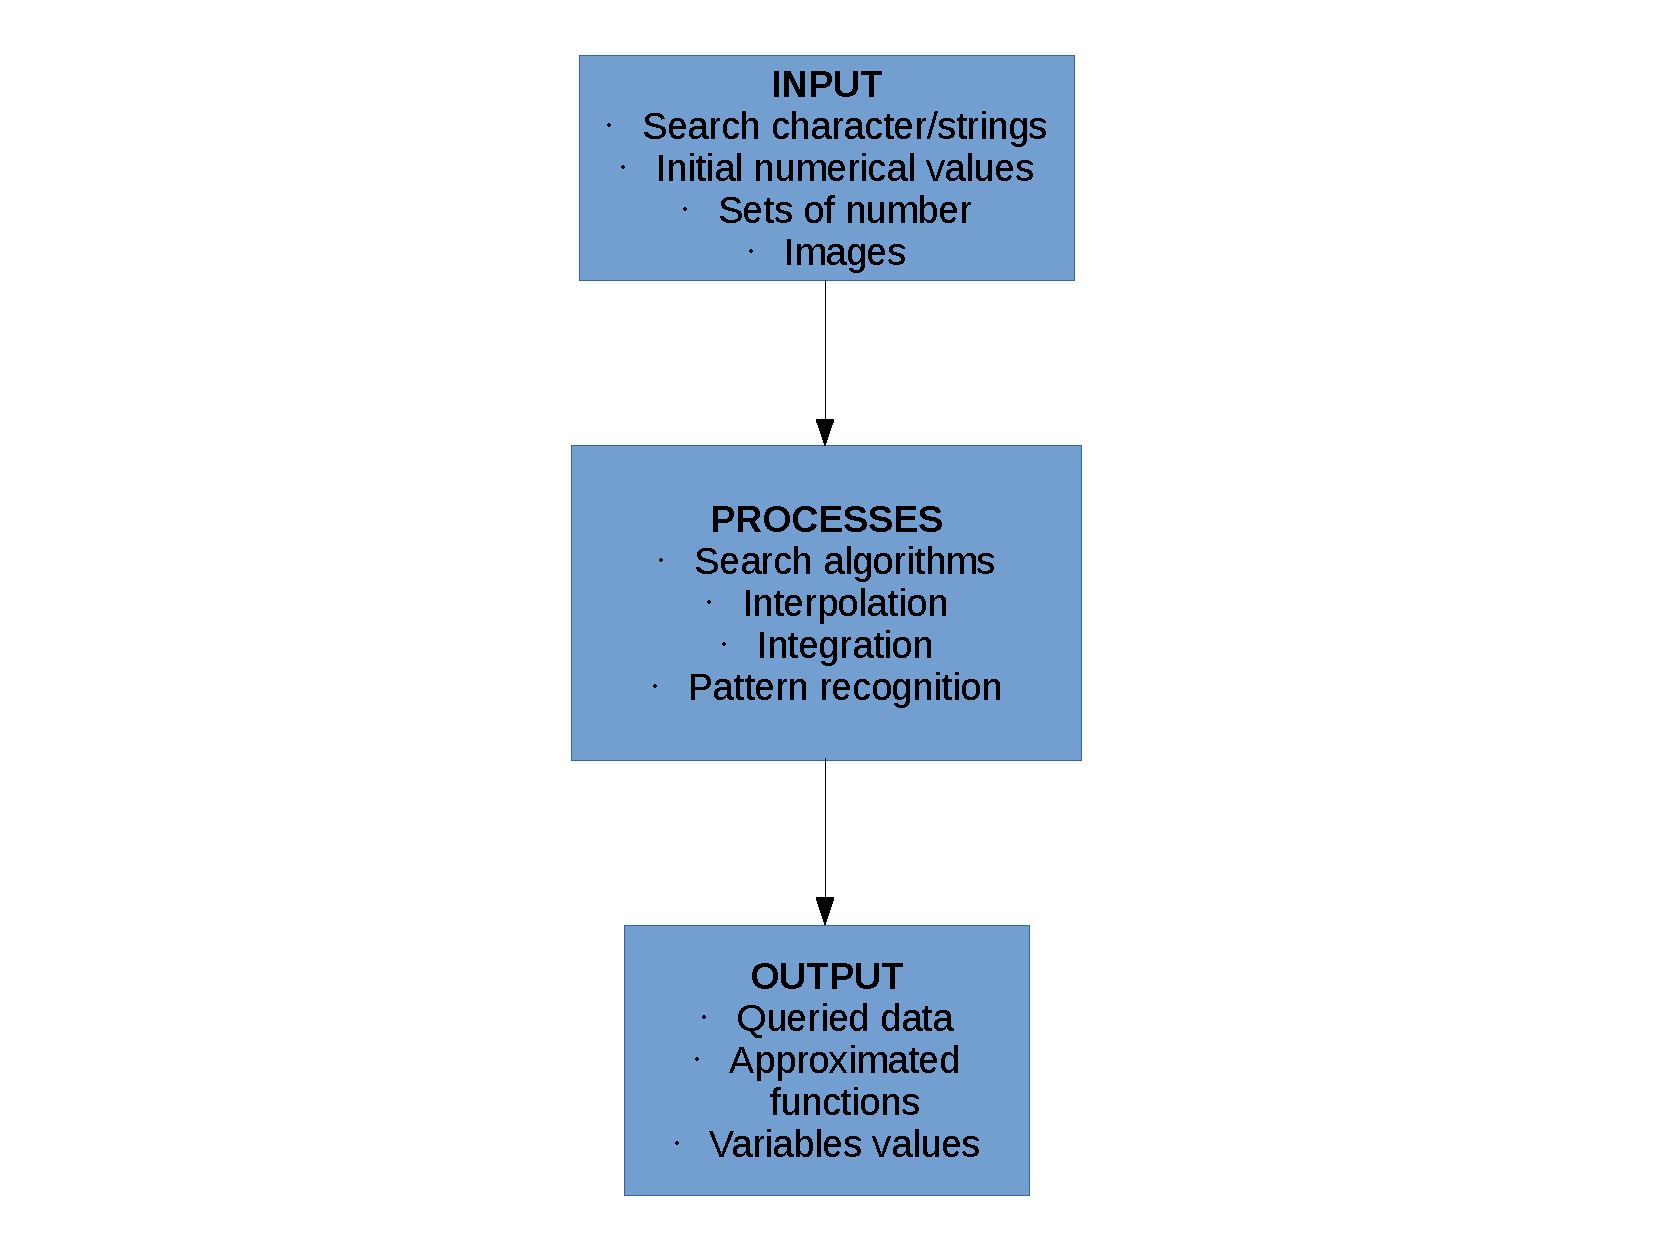
\includegraphics[width=0.8\linewidth]{ProgrammingFlow.pdf}
\end{figure}
\end{frame}

\begin{frame}[fragile]
\frametitle{About programming}
\begin{itemize}
\item Coding paradigm
	\begin{itemize}
	\item programming language == English (sorry, Mandarin not required)
	\item syntax is based on English
	\item coding is a reduction of English instructions
	\end{itemize}

\item Syntax must be remembered
	\begin{itemize}
	\item read the manual $\longrightarrow$ documentations are vital
	\item memorize THE MOST COMMONLY USED syntax only
	\item good algorithm will always beats bad algorithm
	\end{itemize}		

\item I don't remember every syntax so you have to bare with me $\LARGE \pfbox$

\end{itemize}

\end{frame}